\subsection{Vektorer}
Når vektorer omtales, er der tale om en matrice, der kun har en række, kaldet en række vektor, eller en matrice, med kun en søjle, kaldt en søjle vektor. Som reelt anvendes søjle vektorer. \\
Vektorens "koordinator" kaldes komponenter, og antallet af komponenter, kan ses som, hvilken dimension vores vektor har.
\begin{defn}[Søjle vektor]
En \textbf{Søjle vektor} er en matrice med 1 søjle og m rækker, også normalt bare kaldt en vektor.
\begin{align*}
\underset{m \times n}{A} = 
\begin{bmatrix}
a_{1,1}\\
a_{2,1}\\
\vdots \\
a_{m-1,1}\\
a_{m,1} \\
\end{bmatrix}\qquad , n=1\\ %mellemrum skal laves universelt
\end{align*} 
Hvert koordinat kaldes en komponent.
\end{defn}
Hvis et objekt, bliver påvirket af flere forskellige kraft fra forskellige retninger, så er det nødvendigt at vide, hvordan man regner ud hvor objektet bevæger sig hen. Dette gøres ved at sætte vetorene i forlængelse af hinanden, det vil sige at man lægger dem sammen. 
\begin{defn}[Addition af to vektor]
Når to vektor adderes, så adderes de komponenter, som har samme koordinator. Dette kræver, at vektorene har samme antal komponenter.
\begin{align*}
\underset{m \times n}{A} = 
\begin{bmatrix}
a_{1,1}\\
a_{2,1}\\
\vdots \\
a_{m-1,1}\\
a_{m,1} \\
\end{bmatrix}
\qquad
\underset{m \times n}{B} = 
\begin{bmatrix}
b_{1,1}\\
b_{2,1}\\
\vdots \\
b_{m-1,1}\\
b_{m,1} \\
\end{bmatrix}
\qquad , n=1
\end{align*} 
\begin{align*}
A+B=
\begin{bmatrix}
a_{1,1}\\
a_{2,1}\\
\vdots \\
a_{m-1,1}\\
a_{m,1} \\
\end{bmatrix}
+
\begin{bmatrix}
b_{1,1}\\
b_{2,1}\\
\vdots \\
b_{m-1,1}\\
b_{m,1} \\
\end{bmatrix}
=
\begin{bmatrix}
a_{1,1}+b_{1,1}\\
a_{2,1}+b_{2,1}\\
\vdots \\
a_{m-1,1}+b_{m-1,1}\\
a_{m,1}+b_{m,1} \\
\end{bmatrix}
\end{align*}
\end{defn}
\begin{eks}
\textit{Skal måske laves om til 2 komponenter og så en visualisering, eksempel med en båd eller sådan noget}
\begin{align*}
A=
\begin{bmatrix}
4\\
1\\
0\\
-5\\
\end{bmatrix}
\hspace{3cm}
B=
\begin{bmatrix}
7\\
4\\
-2\\
-5\\
\end{bmatrix}\\
A+B=
\begin{bmatrix}
4\\
1\\
0\\
-5\\
\end{bmatrix}
+
\begin{bmatrix}
7\\
4\\
-2\\
-4\\
\end{bmatrix}
=
\begin{bmatrix}
4+7\\
1+4\\
0-2\\
-5-4\\
\end{bmatrix}
=
\begin{bmatrix}
11\\
5\\
-2\\
-9\\
\end{bmatrix}
\end{align*}
\end{eks}
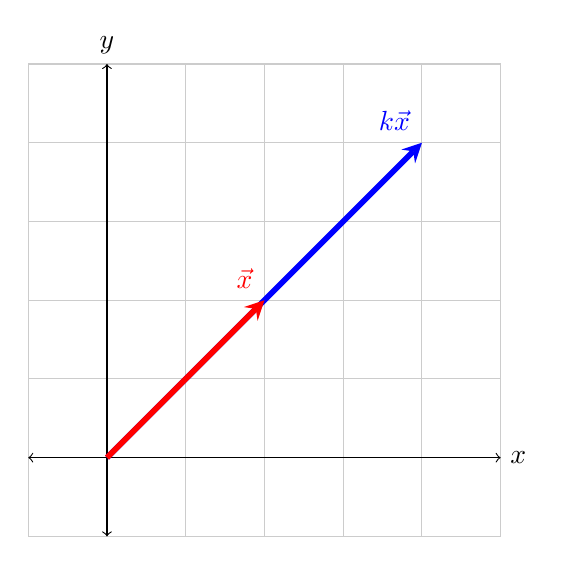
\begin{tikzpicture}
  \draw[thin,gray!40] (-1,-1) grid (5,5); %laver Grid
  \draw[<->] (-1,0)--(5,0) node[right]{$x$}; %x-aksen
  \draw[<->] (0,-1)--(0,5) node[above]{$y$}; %y-aksen
  \draw[line width=2pt,blue,-stealth](0,0)--(4,4) node[above left]{$k\vec{x}$}; %blå vektor
  \draw[line width=2pt,red,-stealth](0,0)--(2,2) node[above left]{$\vec{x}$}; %rød vektor
\end{tikzpicture}
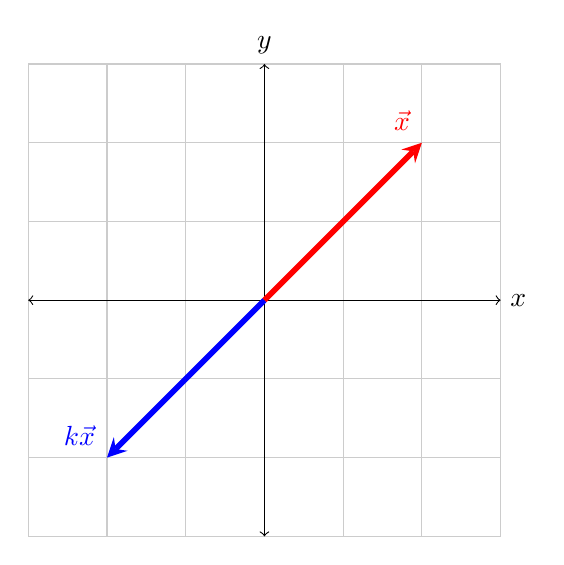
\begin{tikzpicture}
  \draw[thin,gray!40] (-3,-3) grid (3,3);
  \draw[<->] (-3,0)--(3,0) node[right]{$x$};
  \draw[<->] (0,-3)--(0,3) node[above]{$y$};
  \draw[line width=2pt,blue,-stealth](0,0)--(-2,-2) node[above left]{$k\vec{x}$};
  \draw[line width=2pt,red,-stealth](0,0)--(2,2) node[above left]{$\vec{x}$};
\end{tikzpicture}
\begin{defn}[Vektor skalar]
En \textbf{Vektor skalar} er produktet af en vektor $\vec{x}$
som bliver multipliceret med en konstant $k$ kaldet skalar. Denne vektor peger i samme retning, men har en anden længde.
\begin{align*}
\vec{x}=\begin{bmatrix}
x_1\\
x_2\\
\vdots\\
x_{n-1}\\
x_n\\
\end{bmatrix}\\
k\vec{x}=k\begin{bmatrix}
x_1\\
x_2\\
\vdots\\
x_{n-1}\\
x_k\\
\end{bmatrix}=
\begin{bmatrix}
x_1k\\
x_2k\\
\vdots\\
x_{n-1}k\\
x_nk\\
\end{bmatrix}
\end{align*}
\end{defn}
figur 1.5 fra lial
\begin{eks}
En vektor $\vec{x}$ med komponenterne $2$ og $3$ skal skaleres med konstanten $k$ som er $3$, dette gøres ved at multiplicere konstanten med begge komponenter.
\begin{align*}
\vec{x}=\begin{bmatrix}
2\\
3
\end{bmatrix}\qquad k=3\\
k\vec{x}=3
\begin{bmatrix}
2\\
3
\end{bmatrix}
=
\begin{bmatrix}
3\cdot2\\
3\cdot3
\end{bmatrix}
=
\begin{bmatrix}
6\\
9
\end{bmatrix}
\end{align*}
\end{eks}
\subsection{Matrix-vector produkt}

\begin{defn}[Matrix-vektor produkt]
Lad $A$ være en $mxn$ matrice og $x$ være en $nx1$ vektor. Så skrives \textbf{Matrix-vektor produktet} $A\vec{x}$, som er den lineære kombination af rækkerne i $A$ ($\vec{A_j}$) og de tilsvarende komponenter i $\vec{x}$. Dette kræver at matricen har samme antal rækker som vektoren har komponenter(n=j).
\begin{align*}
A\vec{x}=x_1\vec{A}_1+x_2\vec{A}_2+ \dots +x_{n-1}\vec{A}_{n-1}+x_n\vec{A}_n \\
=
\begin{bmatrix}
x_1a_{1 1}+x_2a_{1 2}+\dots +x_{n-1}a_{1 i-1}+x_na_{1 i} \\
x_1a_{2 1}+x_2a_{2 2}+\dots +x_{n-1}a_{2 i-1}+x_na_{2 i}\\
\vdots\\
x_1a_{j-1 1}+x_2a_{j-1 2}+\dots +x_{n-1}a_{j-1 i-1}+x_na_{j-1 i} \\
x_1a_{j 1}+x_2a_{j 2}+\dots +x_{n-1}a_{j i-1}+x_na_{j i}
\end{bmatrix}.
\end{align*}
\end{defn}

\begin{eks}
\begin{align*}
A=
\begin{bmatrix}
1 & 4\\
2 & 5\\
3 & 6
\end{bmatrix}
\qquad
\vec{x}=
\begin{bmatrix}
7\\
8
\end{bmatrix} \\
A\vec{x}= \begin{bmatrix}
1 & 4\\
2 & 5\\
3 & 6
\end{bmatrix}
\begin{bmatrix}
7\\
8
\end{bmatrix}
=
7
\begin{bmatrix}
1\\
2\\
3
\end{bmatrix}
+ 8
\begin{bmatrix}
4\\
5\\
6
\end{bmatrix}=
\begin{bmatrix}
7\\
14\\
21
\end{bmatrix}
+
\begin{bmatrix}
32\\
40\\
48
\end{bmatrix}
=
\begin{bmatrix}
39\\
54\\
69
\end{bmatrix}
\end{align*}
\end{eks}
\begin{defn}[Enhedsvektorer]
\textbf{Enhedsvektorer} er $n$ antal vektorer i $\mathds{R}^n$, som alle har $n$ komponent, hvor en af komponenterne er $1$ og resten $0$
\begin{align*}
A=
\begin{bmatrix}
a_1\\
a_2\\
\vdots\\
a_{n-1}\\
a_n
\end{bmatrix}=
a_1
\begin{bmatrix}
1\\
0\\
\vdots\\
0\\
0
\end{bmatrix}
+
a_2
\begin{bmatrix}
0\\
1\\
\vdots\\
0\\
0
\end{bmatrix}
+
\dots
+a_{n-1}
\begin{bmatrix}
0\\
0\\
\vdots\\
1\\
0
\end{bmatrix}
+
a_n
\begin{bmatrix}
0\\
0\\
\vdots\\
0\\
1
\end{bmatrix}
\end{align*}
\end{defn}